\documentclass{article}

\usepackage{graphicx}
\usepackage{pgf}
\usepackage{tikz}
\usetikzlibrary{shapes,arrows}

\pgfdeclareimage[height=2ex]{lower-bound}{S2_lowerbound}
\pgfdeclareimage[height=2ex]{upper-bound}{S2_upperbound_green}

\begin{document}


\thispagestyle{empty}
\tikzstyle{decision} = [rectangle, draw, fill=yellow!20, text width=.45\textwidth, text badly centered]
\tikzstyle{block} = [rectangle, draw, fill=blue!20,
    text width=.5\textwidth, text centered, rounded corners, minimum height=4em]
\tikzstyle{line} = [draw, thick, -latex']
\tikzstyle{cloud} = [draw, ellipse,fill=blue!20, minimum height=2em]
\def\svgwidth{.8\textwidth}
\definecolor{lowActivity}{rgb}{0.8,0,0}
\definecolor{highActivity}{rgb}{0,0.8,0}%{1,0.8,0}
\newsavebox{\mysquareLow}
\savebox{\mysquareLow}{%
  \raisebox{-0.08em}{%
    \textcolor{black}{%
      \rule{.7em}{.7em}%
    }%
    \hspace{-.65em}%
    \raisebox{.05em}{%
      \textcolor{lowActivity}{%
	\rule{.6em}{.6em}%
      }%
    }%
  }%
}
\newsavebox{\mysquareHigh}
\savebox{\mysquareHigh}{%
  \raisebox{-0.08em}{%
    \textcolor{black}{%
      \rule{.7em}{.7em}%
    }%
    \hspace{-.65em}%
    \raisebox{.05em}{%
      \textcolor{highActivity}{%
	\rule{.6em}{.6em}%
      }%
    }%
  }%
}

\begin{figure}[!ht]
\begin{minipage}{\textwidth}
\centering

\begin{tikzpicture}[node distance = 2cm, auto, scale=0.8, every node/.style={scale=0.8}]
    % Place nodes
    \node [block] (init) {
\begingroup
  \makeatletter
  \providecommand\color[2][]{%
    \errmessage{(Inkscape) Color is used for the text in Inkscape, but the package 'color.sty' is not loaded}
    \renewcommand\color[2][]{}%
  }
  \providecommand\transparent[1]{%
    \errmessage{(Inkscape) Transparency is used (non-zero) for the text in Inkscape, but the package 'transparent.sty'
is not loaded}
    \renewcommand\transparent[1]{}%
  }
  \providecommand\rotatebox[2]{#2}
  \ifx\svgwidth\undefined
    \setlength{\unitlength}{1974.66679688pt}
  \else
    \setlength{\unitlength}{\svgwidth}
  \fi
  \global\let\svgwidth\undefined
  \makeatother
  \begin{picture}(1,0.37)%26031697)%
    \put(0,0){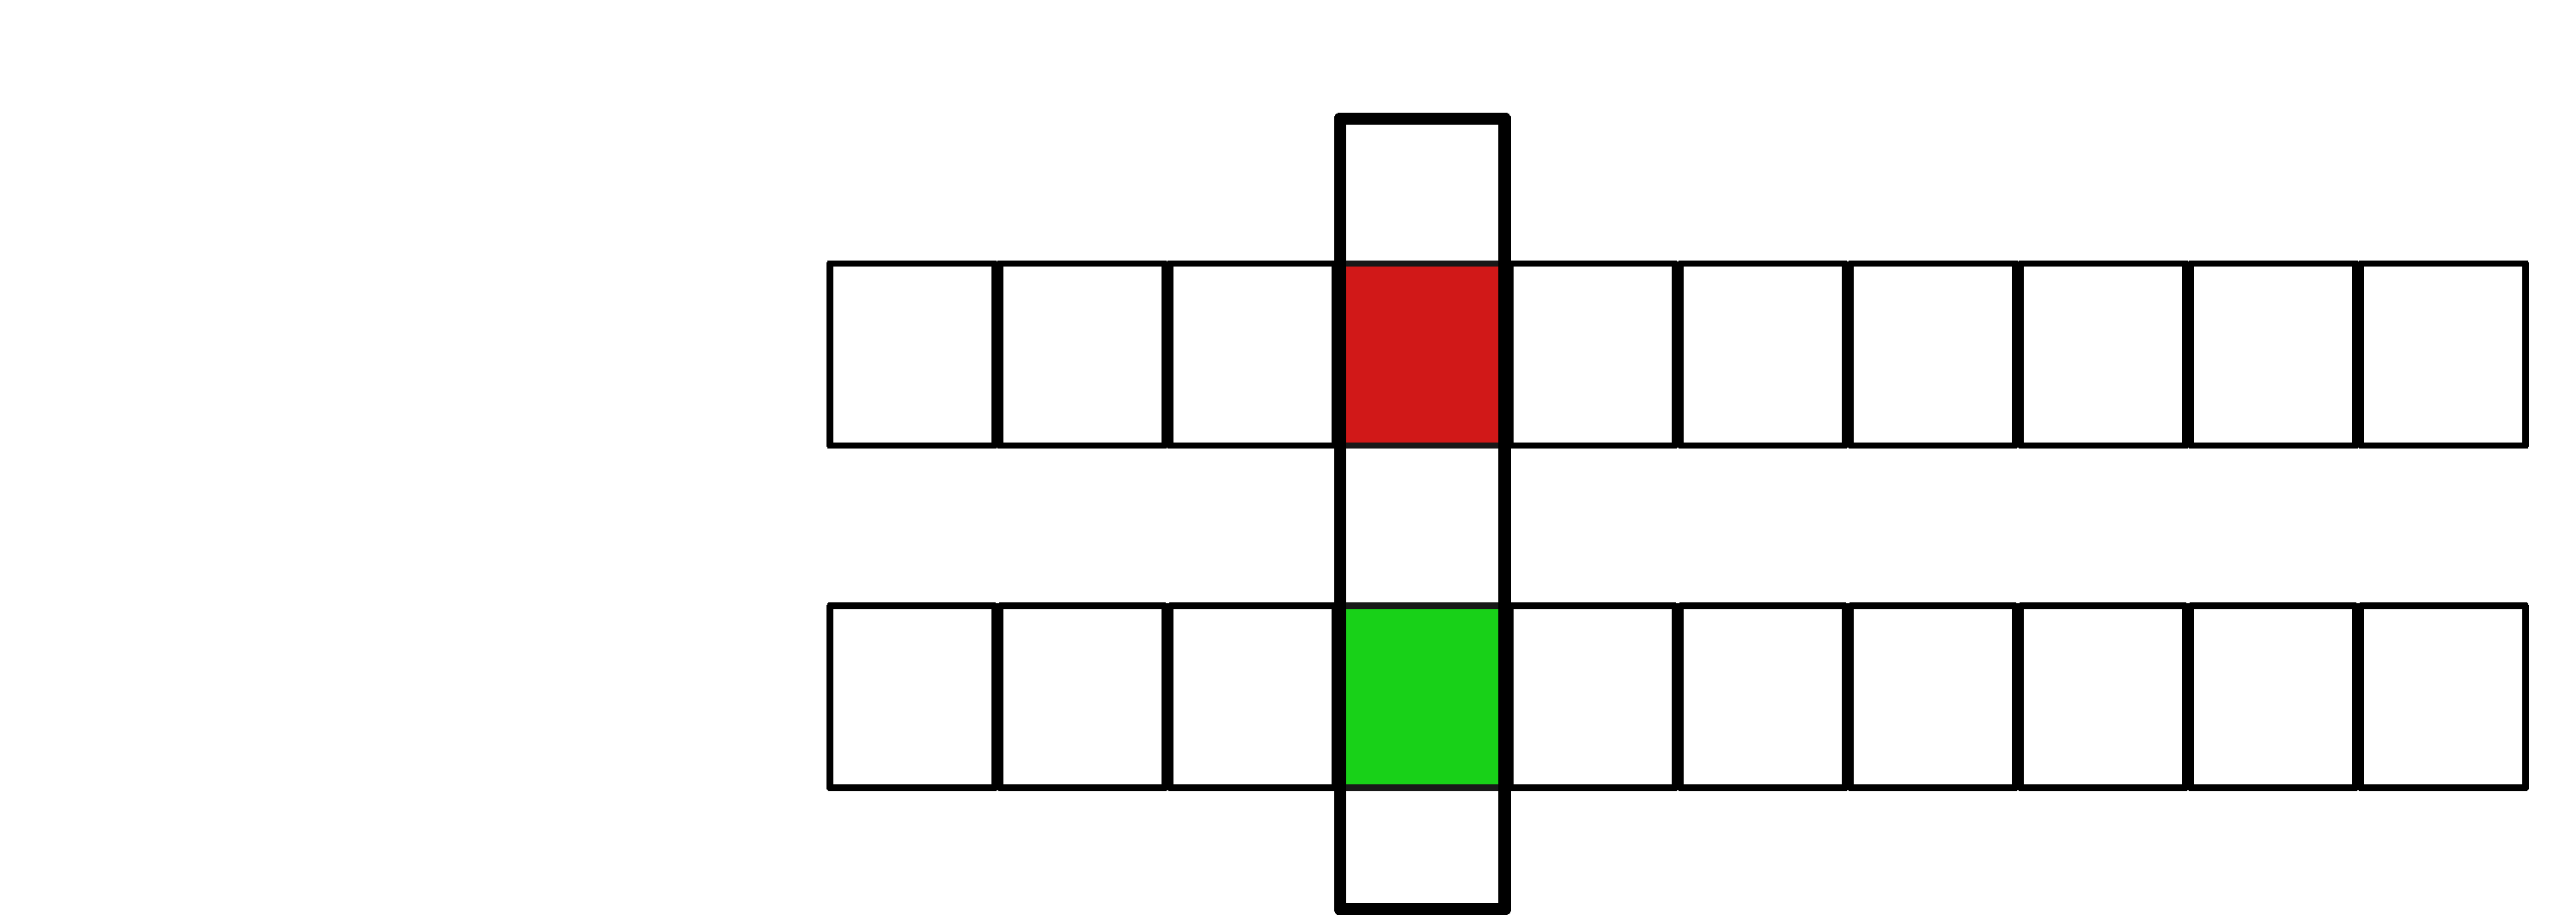
\includegraphics[width=\unitlength]{S2_timeTables.pdf}}%
    \put(-0.08,0.20182345){\color[rgb]{0,0,0}\makebox(0,0)[lb]{\smash{$R_{\mbox{\scriptsize lowerBound}}$}}}%
    \put(-0.08,0.07442319){\color[rgb]{0,0,0}\makebox(0,0)[lb]{\smash{$R_{\mbox{\scriptsize upperBound}}$}}}%
    \put(0.45,0.325)%23815501)
	{\color[rgb]{0,0,0}\makebox(0,0)[lb]{\smash{$\mbox{MEK}_{\mbox{\scriptsize
activity}}$}}}%
  \end{picture}%
\endgroup
};
    \node [block, above of=init, node distance=2.5cm] (reset) {Reset the internal clock: ${\sf t} \!\!:= \!\!0$};
    \node [cloud, above of=reset, node distance=1.5cm] (start) {Start};
\node [block, below of=init, node distance=2.5cm] (choose) {$R$ will occur when
\raisebox{-0.3ex}{\pgfuseimage{lower-bound}} $\leq\!\!\! {\sf t}\!\!\! \leq$
\raisebox{-0.3ex}{\pgfuseimage{upper-bound}}
    };
    \node [block, below of=choose] (increase) {Increase $\mbox{ERK}_{\mbox{\scriptsize activity}}$
by $+1$ level};
    \node [block, below of=increase] (inform) {Inform interactions \mbox{depending} on $\mbox{ERK}_{\mbox{\scriptsize
activity}}$ 
    of the change};
    % Draw edges
    \path [line] (start) -- (reset);
    \path [line] (reset) -- (init);
    \path [line] (init) -- (choose);
    \path [line] (choose.west) -| +(-0.5, 2) node [pos=0.78, sloped, above, align=left] {$\mbox{MEK}_{\mbox{\scriptsize activity}}$ was changed} |- (init.west);
    \path [line] (choose) -- (increase);
    \path [line] (increase) -- (inform);
    \path [line] (inform.east) -| +(1, 4) |- (reset.east);
\end{tikzpicture}
\end{minipage}
\end{figure}

\end{document}